\chapter{Les Projets}
\label{Developpement}

\section{MobiSAAS}

\subsection{Présentation}

Le projet "MobiSAAS" : MobiAnalyst as a Service, s'inscrit dans la démarche d'entreprise de proposer des solutions en mode \textbf{SAAS}. Le projet consiste d'une manière générale à exposer les fonctionnalités de la solution desktop du produit "MobiAnalyst"(Fig. \ref{OffreMobiAnalyst}).\\

\begin{figure}[!h]
\centering
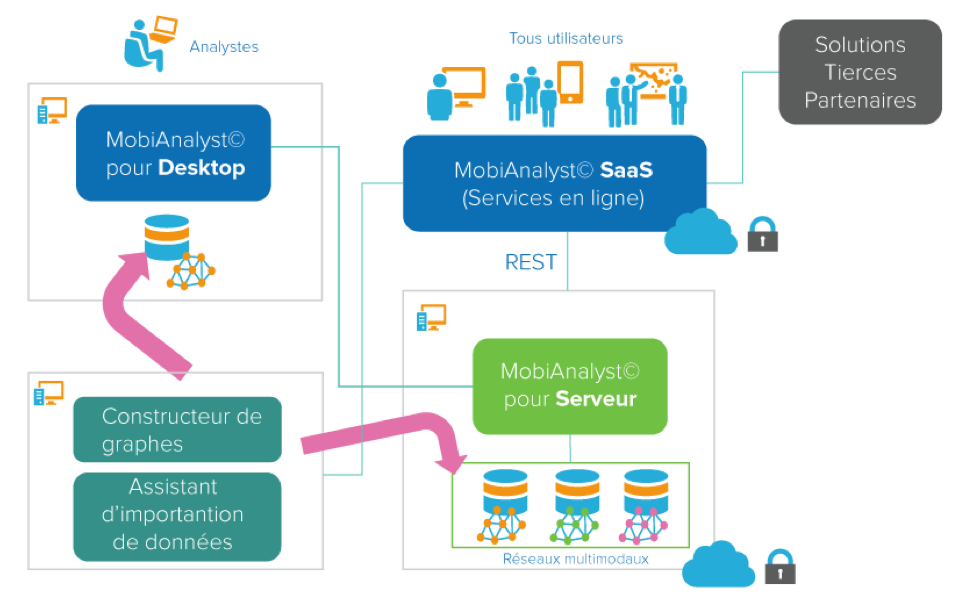
\includegraphics[width=14cm]{images/offre_MobiAnalyst.png}
\caption{\label{OffreMobiAnalyst}Offre du produit MobiAnalyst}
\end{figure} 

\subsection{Eléments de spécifications fonctionnelles et techniques}

\subsubsection{Architecture actuelle}

La figure \ref{fig:architecture} détaille l'ensemble des briques logicielles nécessaires au fonctionnement de la plate-forme MobiSAAS :
\begin{itemize}
\item \textbf{AGS} : ArcGIS Server. Le serveur de Système d'Information Géographique (SIG) permettant de publier et d'administrer des services cartographiques (MapService).
Dans notre cas, les MapServices déployés sont des réseaux routiers et de transport en commun (TC), accompagnés de tables horaires (TimeTable) contenant les horaires des TC.
\item \textbf{SOE}: Server Object Extension. Nous utilisons le mécanisme d'extension "SOE" pour déployer sur un MapService un service spécifique à MobiSAAS. Un SOE est une fonctionnalité qui se déploie sur un MapService et qui expose en Web Service (REST ou SOAP) les solveurs (algorithme de résolution d'itinéraires) de MobiAnalyst.
\item \textbf{MobiAdmin}: Serveur REST d'administration MobiSAAS. Ce serveur (basé sur Java) est le point d'entrée des utilisateurs des services REST de MobiAnalyst.
Il redirige les requêtes métiers vers le bon SOE déployé, il trace ces requêtes et enrichit la base de données client de MobiAnalyst.
L'authentification qui est faite dans les requêtes utilise les comptes d'AGS créés au préalable.
\item \textbf{Postgres} : Système de gestion de base de données. Cette base contient les données clients de MobiAnalyst : profil, traces d'utilisation de MobiSAAS.
\item \textbf{MongoDB} : Système de gestion de base de données. Cette base contient les logs (statistiques mesurées en temps réel) correspondant aux services REST de MobiSAAS.
\end{itemize}

\begin{figure}[h]
	\centering
		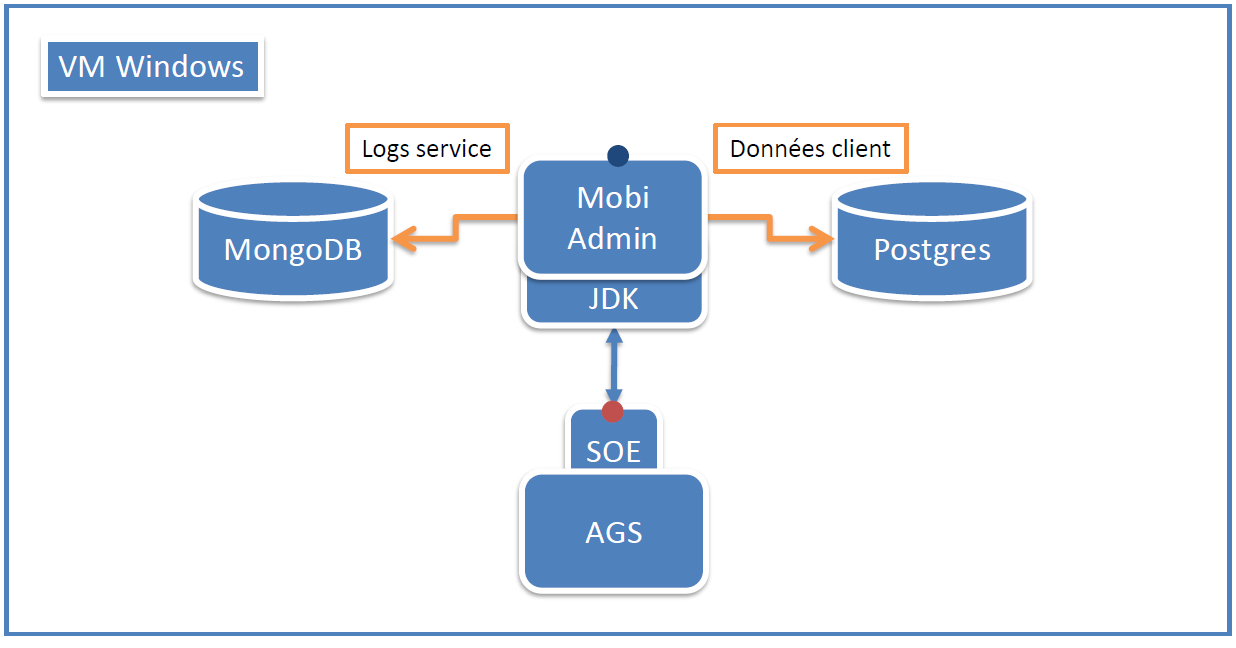
\includegraphics[width=0.8\textwidth]{images/architecture.png}
	\caption{Architecture globale.}
	\label{fig:architecture}
\end{figure}\\

Pour le composant "MobiAdmin" le choix technologique majeur est d'utiliser le framework DropWizard (cf. Annexe \ref{Annexe B}). Ce framework orienté micro-services nous permet de fournir notamment un serveur embarqué HTTP "Jetty". Jersey pour la partie webservice REST qui est l'implémentation de référence de la spécification JAX-RS. Ou encore Jakson pour la dé/sérialisation du JSON.\\


\subsection{Développements}

Mon stage et les développements demandés concernent le composant d'administration de l'infrastructure : "MobiAdmin". Dans l'objectif de gérer les données du client, je dois proposer un service de gestion des données de transport dans l’espace privatif du client.
La fonctionnalité principale à développer est un "Upload de données" et plus particulièrement l'upload de données GTFS\footnote{\url{https://developers.google.com/transit/gtfs/reference}}.\\ 

L'objectif de ce service d'import de données GTFS est de pouvoir manipuler ces données (fichier au format zip) (comme le fait le DataWizard) et ainsi pouvoir récupérer des métadonnées ex: l'extension géographique des données, le nom de l'agence, le nombre de lignes, le mode de transport,...\\
Une archive "Upload" peut contenir un seul ou plusieurs jeu de données GTFS (ensemble de fichiers .txt). Il faut donc récupérer et renseigner les métadonnées de chaque upload de fichier :
\begin{itemize}
\item Nom 
\item Date d’upload ou de la version du GTFS
\item Licence (open data/ restreint/ privé)
\item Url si open data
\item Commentaire libre
\item Chemin vers la données
\item etc...
\end{itemsize}\\

L'environnement de développement est donc un projet Java EE Maven composé des éléments de Dropwizard. \\
Ces WS sont à priori “lourds”, sachant qu'un jeu de données peut faire jusqu'à plusieurs centaines de Mo, les opérations de téléchargement, validation, traitement, stockage dans en base,... vont être long à renvoyer une réponse au client après chaque requête. Les WS à développer sont donc asynchrones. De plus, une contrainte supplémentaire et que le service doit supporter plusieurs requêtes simultanées, il faudra donc s'orienter vers un développement en mode "programmation concurrente".\\


\subsection{Résultats obtenus / Difficultés rencontrées}

J'ai tout d'abord commencé par découvrir Maven (cf. Annexe \ref{Annexe A}), les projets, les modules, le désormais célèbre fichier \textbf{POM}, etc...
Ensuite, je me suis documenté sur le code métier existant, et chercher des outils ou librairies de professionnels du domaine (cf. Outils métiers \ref{OBA}).
Enfin, après le "Getting Started" de Dropwizard\footnote{\url{https://dropwizard.github.io/dropwizard/getting-started.html}}, une fois tout cela bien maîtrisé, j'ai pu  commencé la conception et le développement de services web REST.\\

J'ai choisit de stocker les informations concernant ma partie de l'application dans une table PostgreSQL (Fig \ref{TablePostgres})\\
\begin{figure}[!h]
\centering
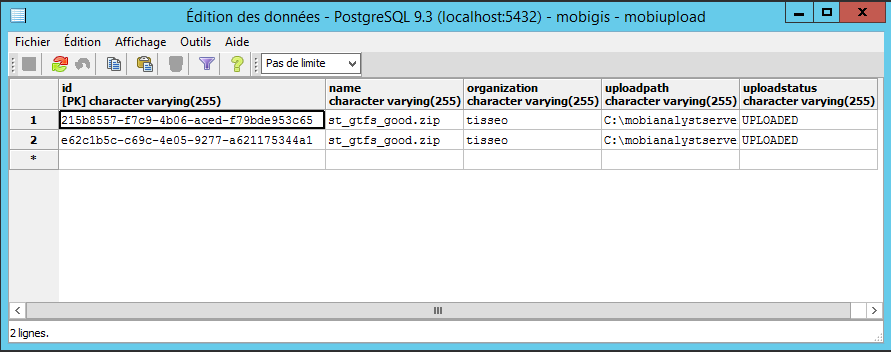
\includegraphics[width=14cm]{images/tablePostgres_mobiupload_small.png}
\caption{\label{TablePostgres}Table des uploads sur le SGBD PostgreSQL}
\end{figure} 

A chaque requête POST du client, je créé une instance d'objet Upload, les informations sont saisies dans la table de suivi, et je stocke les données envoyées sur le serveur. Pour chaque client ou utilisateur, pour chaque type de données, il y a un répertoire personnalisé, chaque upload est "taggé" d'un identifiant unique "UUID".
Le code métier qui a été implémenté est pour le moment le test sur le type de données envoyées, la validation des données et la production d'un rapport d'un validation (JSON), enfin l'extraction (récursive) des données contenues dans l'archive(cf. Annexe \ref{Annexe D}).\\

\subsection{Perspectives}

L'idéal d'un programme développé dans un langage orienté objet, est la généricité, et la réutilisation d'un maximum de composants. Dans ce travail, l'objectif est clairement de produire un maximum de composant abstrait (classes et interfaces) et de méthodes réutilisables. Les perspectives du projet "MobiSAAS" sont nombreuses : gérer une architecture distribuée, augmenter les fonctionnalités SAAS notamment les principales du projet "DataWizard".\\

J'ai donc débuté le développement de ces composants abstraits (ex: Les ressources au sens DropWizard (Fig. \ref{UML1}). Grâce à cela on pourra donc "uploader" plusieurs types de données et réutiliser la méthode manageUpload(). Egalement, sur ce même principe j'ai développé une classe abstaite afin de faire proposer la gestion des threads et tous mes services en hérite, cela limite la duplication de codes dans l'application.\\
\begin{figure}[!h]
\centering
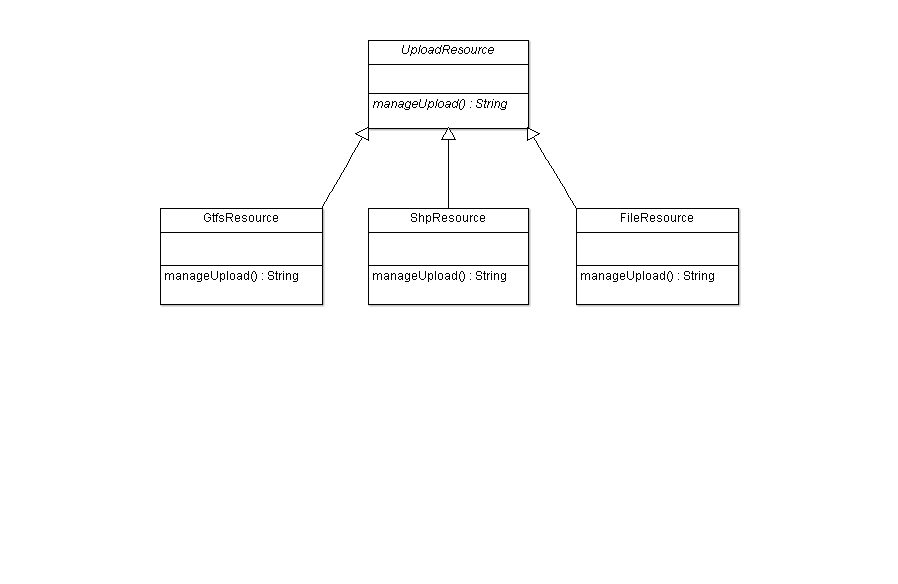
\includegraphics[width=14cm]{images/Diagrammedeclasses_heritage_full.png}
\caption{\label{UML1}Exemple d'abstraction et d'héritage de méthode}
\end{figure} 



\section{DataWizard}

\subsection{Présentation}

Le projet "DataWizard", ensemble de scripts Python et SQL est une application dont le but est d'ingérer des données de transports, et de voirie dans une base de données spatiales (\textbf{PostgreSQL/PostGIS}\ref{Postgis}) afin de produire en sortie un réseau de transport (Network Dataset ou NDS).\\


\subsection{Eléments de spécifications fonctionnelles et techniques}

Le DataWizard permet de se lancer par étapes. Il y a 10 étapes successives, dont une étape préliminaire appelée étape 0, et une indépendante : l'étape 10.
\begin{itemize}
\item STEP 0 : Nettoyage et préparation de la base de données
\item STEP 1 : Import des données transport en commun et conversion vers le schéma mobianalyst
\item STEP 2 : Import des données de voirie
\item STEP 3 : Import des données métro et conversion vers le schéma mobianalyst
\item STEP 4 : Génération des données vitesses moyennes et horaires et connexion des réseaux de transport en commun et voirie
\item STEP 5 : Calcul des horaires et des vitesses moyennes
\item STEP 6 : Export des données vers des fichiers Shapefile (.shp)
\item STEP 7 : Import des données dans la Géodatabase de sortie et changement du système de projection si nécessaire
\item STEP 8 : Extraction des différents modes, génération du fichier xml servant à construire le réseau et de MobiNetwork.xml
\item STEP 9 : Construction et compilation du réseau
\item STEP 10 : Production de métadonnées pour le réseau
\end{itemize}

Afin de fournir, un réseau conforme aux attentes du logiciel MobiAnalyst "version 3.0" et des experts en analyse de réseaux de transports, l'équipe me fournit une spécification de métadonnées à extraire des données en entrée du DataWizard (Fig. \ref{DW_Metadata}).\\

\begin{figure}[!h]
\centering
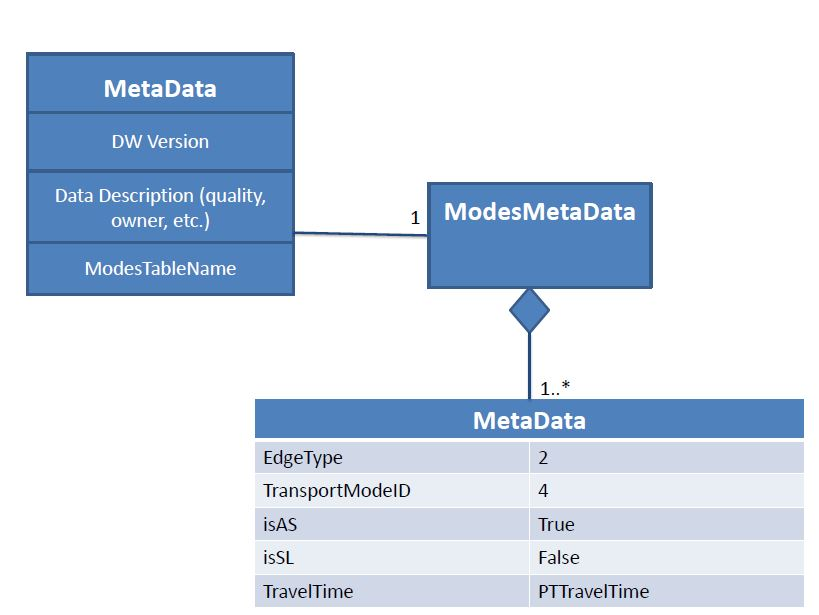
\includegraphics[width=14cm]{images/DW_specMetadata.JPG}
\caption{\label{DW_Metadata}Schéma des tables de métadonnées}
\end{figure} 

\subsection{Développements}

J'intègre tout d'abord le projet en tant qu'utilisateur, j'exploite des données et produits des réseaux (Bordeaux, Champagne-Ardennes, Montreal, Melbourne,etc...) Ensuite, petit à petit je suis le plan de charge issu du projet Redmine et corrige des bugs, et anomalies.\\

Mon premier travail a été de développer l'étape 10 (STEP 10 : Export Metadata Tables) de l'exécution du DataWizard. Pour cela j'ai du extraire le nombre de mode de transports en commun (variable selon chaque projet), leur code (variable selon chaque projet) et enfin extraire des listes de constantes pour documenter le réseau produit par le DataWizard.\\

Exemple ?\\

Un autre travail réalisé est le développement qui permet la gestion du système de projection des données géographiques pour les calculs du DataWizard. Cette modification impacte quasiment la totalité des requêtes SQL dites spatiales de l'application, et permet des résultats (calculs de distances) plus réalistes (par exemple pour Melbourne, Australie située dans l'hémisphère Sud).\\


\subsection{Résultats obtenus / Difficultés rencontrées}

Les principales difficultés concernent les données. Ces données sont complexes, les données GTFS ou les données de voirie (données Here (anciennement Navteq) ou OpenStreetMap\footnote{\url{http://openstreetmap.fr/}}). La base de données "DataWizard" possède ainsi de nombreux schémas, et les requêtes SQL sont parfois très complexes mêlant fonctions, et requêtes géographiques.\\

Les résultats obtenus sont la production de nombreux réseaux en version 3.0 (avec les métadonnées) pour nos analystes, et pour les projets nécessitant des réseaux récents (Moveazy, Mobilyse, etc...). Et une version de l'application qui je l'espère est plus stable.\\

Dans ce projet, j'ai également développé des fonctions utilitaires : BOMConverter.py, searchAndReplaceFiles.py, etc... Ces méthodes permettent notamment de formater les données avant leur import dans la base de données. Cela peut certainement éviter les mauvaises surprises d'encodage ou de caractères spéciaux fréquemment rencontrés lors de l'exploitation de données GTFS.\\


\subsection{Perspectives}

La liste des évolutions est longue, il y a en effet énormément de perspectives pour le projet... Tout d'abord permettre l'import de plusieurs formats de données, comme l'import de données Shapefile, mais aussi de données de transports en commun "Trident"...
Mais aussi d'une manière générale optimiser les étapes, et développer des routines de simplification de données (afin de ne retenir que les données nécessaires),...\\

